A teszter elkészítése után a rendszer tesztelése következett.
A rendszer nem fektetett nagy hangsúlyt a pontosságra, viszont egy 
megközelítő értéket meg kell tudjon határozni.

\section{Ellenállás mérés}

Amennyiben az elkatrész egy ellenállás akkor meghatározza ennek az ellenállását.
Mivel az ADC-n levő konstans és változó zajok vannak és ezen alapszik 
az áramerősség mérése, így a mérések pontossága nem magas[\ref{fig:ResistorResults}], ami különösen csökken a mérés tartomány
végén, mivel a mérő ellenállás amit az áramerősség mérésére használ túl alacsony így
nem képes pontosan meghatározni az áramerősséget. Ezt egy nagyobb mérő ellenállással
lehetne korrigálni.


\begin{table}[H]
    \begin{tabular}{|l|l|l|l|}
    \hline
    Sorszám & Névleges érték(Ohm) & Multiméterrel mért érték(Ohm) & Teszter által mért érték(Ohm) \\ \hline
    0       & 47             & 47                       & 52.5                     \\ \hline
    1       & 56             & 55.7                     & 59                       \\ \hline
    2       & 100            & 100.1                    & 107.4                    \\ \hline
    3       & 220            & 218                      & 242                      \\ \hline
    4       & 360            & 356                      & 398                      \\ \hline
    5       & 540            & 544                      & 606                      \\ \hline
    6       & 1000           & 980                      & 890                      \\ \hline
    7       & 2200           & 2198                     & 2301.7                   \\ \hline
    8       & 4700           & 4670                     & 4319.7                   \\ \hline
    9       & 10000          & 9680                     & 9237                     \\ \hline
    10      & 33000          & 32660                    & 28305.7                  \\ \hline
    11      & 62000          & 62000                    & 49590                    \\ \hline
    \end{tabular}
    \end{table}

    \begin{figure}[H]
        \centering
        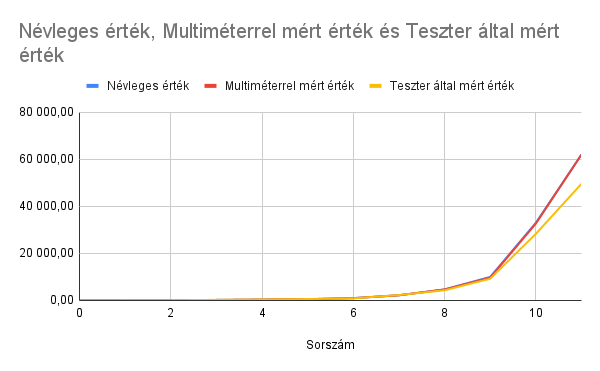
\includegraphics[scale=0.6]{images/results/resistorMesurement.png}
        \caption{Ellenállás mérés eredménye}
        \label{fig:ResistorResults}
    \end{figure}

    A tesztelés relatív hibája alább látható[\ref{fig:ResistorRelErrorResults}].
    \begin{figure}[H]
        \centering
        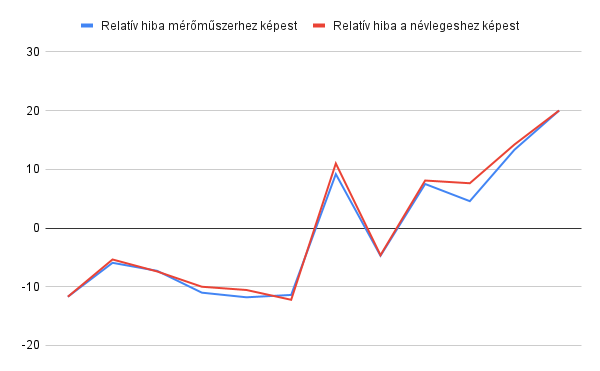
\includegraphics[scale=0.6]{images/results/RelErrorResistor.png}
        \caption{Ellenállás mérés relatív hibája}
        \label{fig:ResistorRelErrorResults}
    \end{figure}


\section{Kondenzátor}

Kondenzátor mérés estén az időt méri ameddig a kondenzátor feszültsége eléri a 
68\%-át a 3.3V-os forrásnak. Ezen esetben a mérés pontosabb, mivel
a zajok kevésbé befolyásolják így nem kell alacsony értékekből
számolni ami nagy hibához vezet. 50nF alatt nem biztos a mérés, 
mivel egyes alkatrészeket másnak is detektálhat, különösen ha 
hosszú vezetékek vannak használva. A grafikonon[\ref{fig:ResistorResults}]
látható, hogy a mérés jól megközelíti a névleges és dedikált mérőműszer
eredményeit.

\begin{table}[H]
    \begin{tabular}{|l|l|l|l|}
    \hline
    sorszám & Névleges érték & Mérőműszerrel mért érték & Mért érték \\ \hline
    1       & 60nF           & 59.62nF                  & 60nF       \\ \hline
    2       & 75nF           & 74.26                    & 75nF       \\ \hline
    3       & 100nF          & 98.26nF                  & 101nF      \\ \hline
    4       & 200nF          & 202nF                    & 203nF      \\ \hline
    5       & 300nF          & 300.3nF                  & 305nF      \\ \hline
    6       & 400nF          & 400nF                    & 406nF      \\ \hline
    7       & 500nF          & 498nF                    & 504nF      \\ \hline
    8       & 600nF          & 602nF                    & 610nF      \\ \hline
    9       & 700nF          & 701nF                    & 703nF      \\ \hline
    10      & 800nF          & 791.4nF                  & 800nF      \\ \hline
    11      & 900nF          & 889.7nF                  & 889nF      \\ \hline
    12      & 1uF            & 979nF                    & 1.059uF    \\ \hline
    13      & 2uF            & 1.97uF                   & 2.033uF    \\ \hline
    14      & 3uF            & 2.95uF                   & 3.05uF     \\ \hline
    15      & 4uF            & 3.96uF                   & 4.025uF    \\ \hline
    16      & 5uF            & 4.94uF                   & 5uF        \\ \hline
    17      & 6uF            & 5.935uF                  & 6.016uF    \\ \hline
    18      & 7uF            & 6.914uF                  & 6.95uF     \\ \hline
    19      & 8uF            & 7.946uF                  & 8.05uF     \\ \hline
    \end{tabular}
    \end{table}

    \begin{figure}[H]
        \centering
        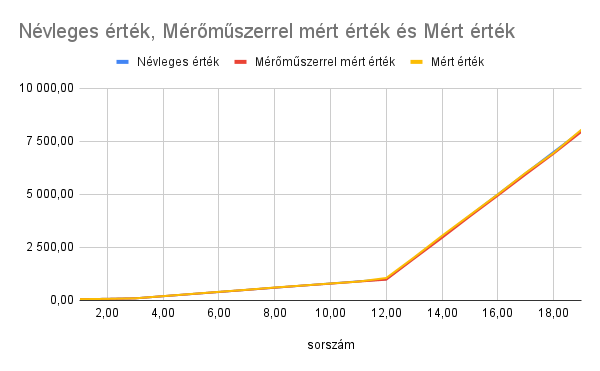
\includegraphics[scale=0.6]{images/results/CapacitorMeasurement.png}
        \caption{Kondenzátor mérés eredménye}
        \label{fig:CapacitorResults}
    \end{figure}

    A tesztelés relatív hibája alább látható[\ref{fig:CapRelErrorResults}].

    \begin{figure}[H]
        \centering
        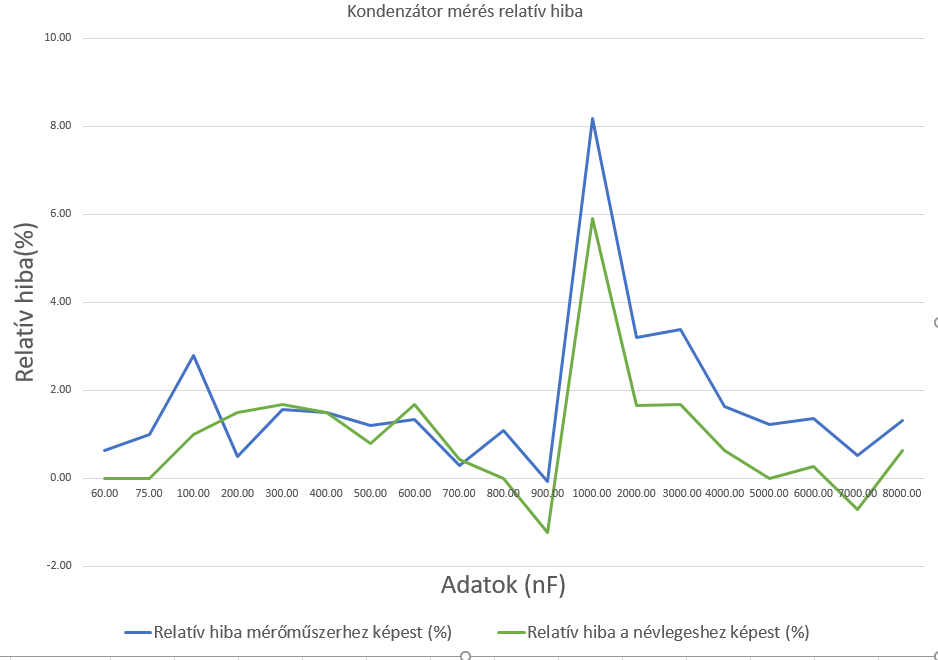
\includegraphics[scale=0.6]{images/results/CapRelError.png}
        \caption{Kondenzátor mérés relatív hibája}
        \label{fig:CapRelErrorResults}
    \end{figure}

\section{Dióda}

A dióda mérés a diódán eső feszültséget méri miközben az egyik oldala
tápfeszültségen van és a kapcsoló ellenállások használatával.
A mérések során azt tapasztaltam, hogy a multiméter alacsonyabb
értékeket adott, míg a teszter nagyobbakat, viszont a LED-ek
tesztelése során világosabban villant fel. Így arra a következtetésre
jutottam, hogy a multiméter azt a feszültséget mérte ahol
minimálisan elkezdett a dióda vezetni és a teszter meg amikor
már teljesen nyitva van. A kék LED esetében a multiméter nem volt képes
megmérni a nyitó feszültséget, viszont ez 2.5 és 3.7V közt helyezkedhet el.

2 inverz diódát is képes megmérni, ebben az esetben azt adja vissza, hogy melyik
irányban mekkora a dióda nyitó feszültsége.

\begin{table}[H]
    \begin{tabular}{lll}
    Sorszám                 & Mérőműszerrel mért érték                  & Mért érték                \\ \hline
    \multicolumn{1}{|l|}{0} & \multicolumn{1}{l|}{0,54}                 & \multicolumn{1}{l|}{0,69} \\ \hline
    \multicolumn{1}{|l|}{1} & \multicolumn{1}{l|}{1,58}                 & \multicolumn{1}{l|}{1,8}  \\ \hline
    \multicolumn{1}{|l|}{2} & \multicolumn{1}{l|}{1.85}                 & \multicolumn{1}{l|}{1,96} \\ \hline
    \multicolumn{1}{|l|}{3} & \multicolumn{1}{l|}{1,78}                 & \multicolumn{1}{l|}{2,01} \\ \hline
    \multicolumn{1}{|l|}{4} & \multicolumn{1}{l|}{kék LED, nem mérhető} & \multicolumn{1}{l|}{2,83} \\ \hline
\end{tabular}
\end{table}

\section{Tranzisztor}

Ebben az esetben a teszter megméri a tranzisztor lábkiosztását és az erősítését.
Képes az emitter és kollektor különbséget is meghatározni az erősítés nagyságából,
mivel az erősítés nagyobb abban az esetben, amikor a tranzisztor a helyes irányban
vezeti az áramot (NPN esetében az áram a kollektor emitter úton folyik).
Az erősítést akkor méri, amikor a tranzisztor kinyit, de még nincs teljesen kinyitva,
hanem a kollektor-emitter feszültség 2V körül van. Ezt a bázis feszültség
értékének a szabályozásával érhető el. Ekkor megméri a kollektor áramot
(mivel itt még nincs meghatározva, hogy melyik az, így most az ahonnan
az áram folyik) és elossza a bázison levő árammal.

Egy hiba a mérések alatt az volt, hogy a bázisra kis ellenállást
kapcsoltam és a tranzisztort a saturációs pontba tettem ahol 
nagy áram folyt a bázison keresztül ezért az erősítése nagyon alacsony
(5 alatt) volt, míg nagyobb ellenállással sem volt képes megközelíteni
az adatlapi értékét ebben az esetben. Amíg az új verzióval az 
erősítés sokkal jobban megközelíti a valóságot.

\section{Karakterisztika diagram}


\subsection{Kimeneti karakterisztika}

Az áramerősséget azon az értéken hagyva ahol a tranzisztor elkezdett kinyitni
végig mér a C-E feszültség 0-3.3V-os tartományán. A bázis használ egy 
P szabályozót, mivel a rendszer csak konstans feszültség forrást tartalmaz
és nem áramot. Az áram referencia ebben az esetben amikor a kollektor
emitter feszültsége eléri az 1.5V-ot

Minden mérési pontban megméri a kollektor
áramerősséget. Ezeket az eredményeket elmenti, majd kirajzolja a 
teszteren található kijelzőre. A kirajzolás csak a kijelzőn
jelenik meg, mivel egy egyszerű Serial port olvasó program
szöveg megjelenítésére használatos és nincs számítógép oldani applikáció.

A PNP tranzisztor esetében az emitter konstans 3.3V-on tartásával és 
kollektor csökkentésével 3.3V-ról a emitter-kollektor feszültség
0 és 3.3V közt változik, miközben a bázis feszültsége sosem negatív
a földhöz képest.

A mérés a következőképpen lesz látható a kijelzőn[\ref{fig:OutChar}] 

\begin{figure}[H]
    \centering
    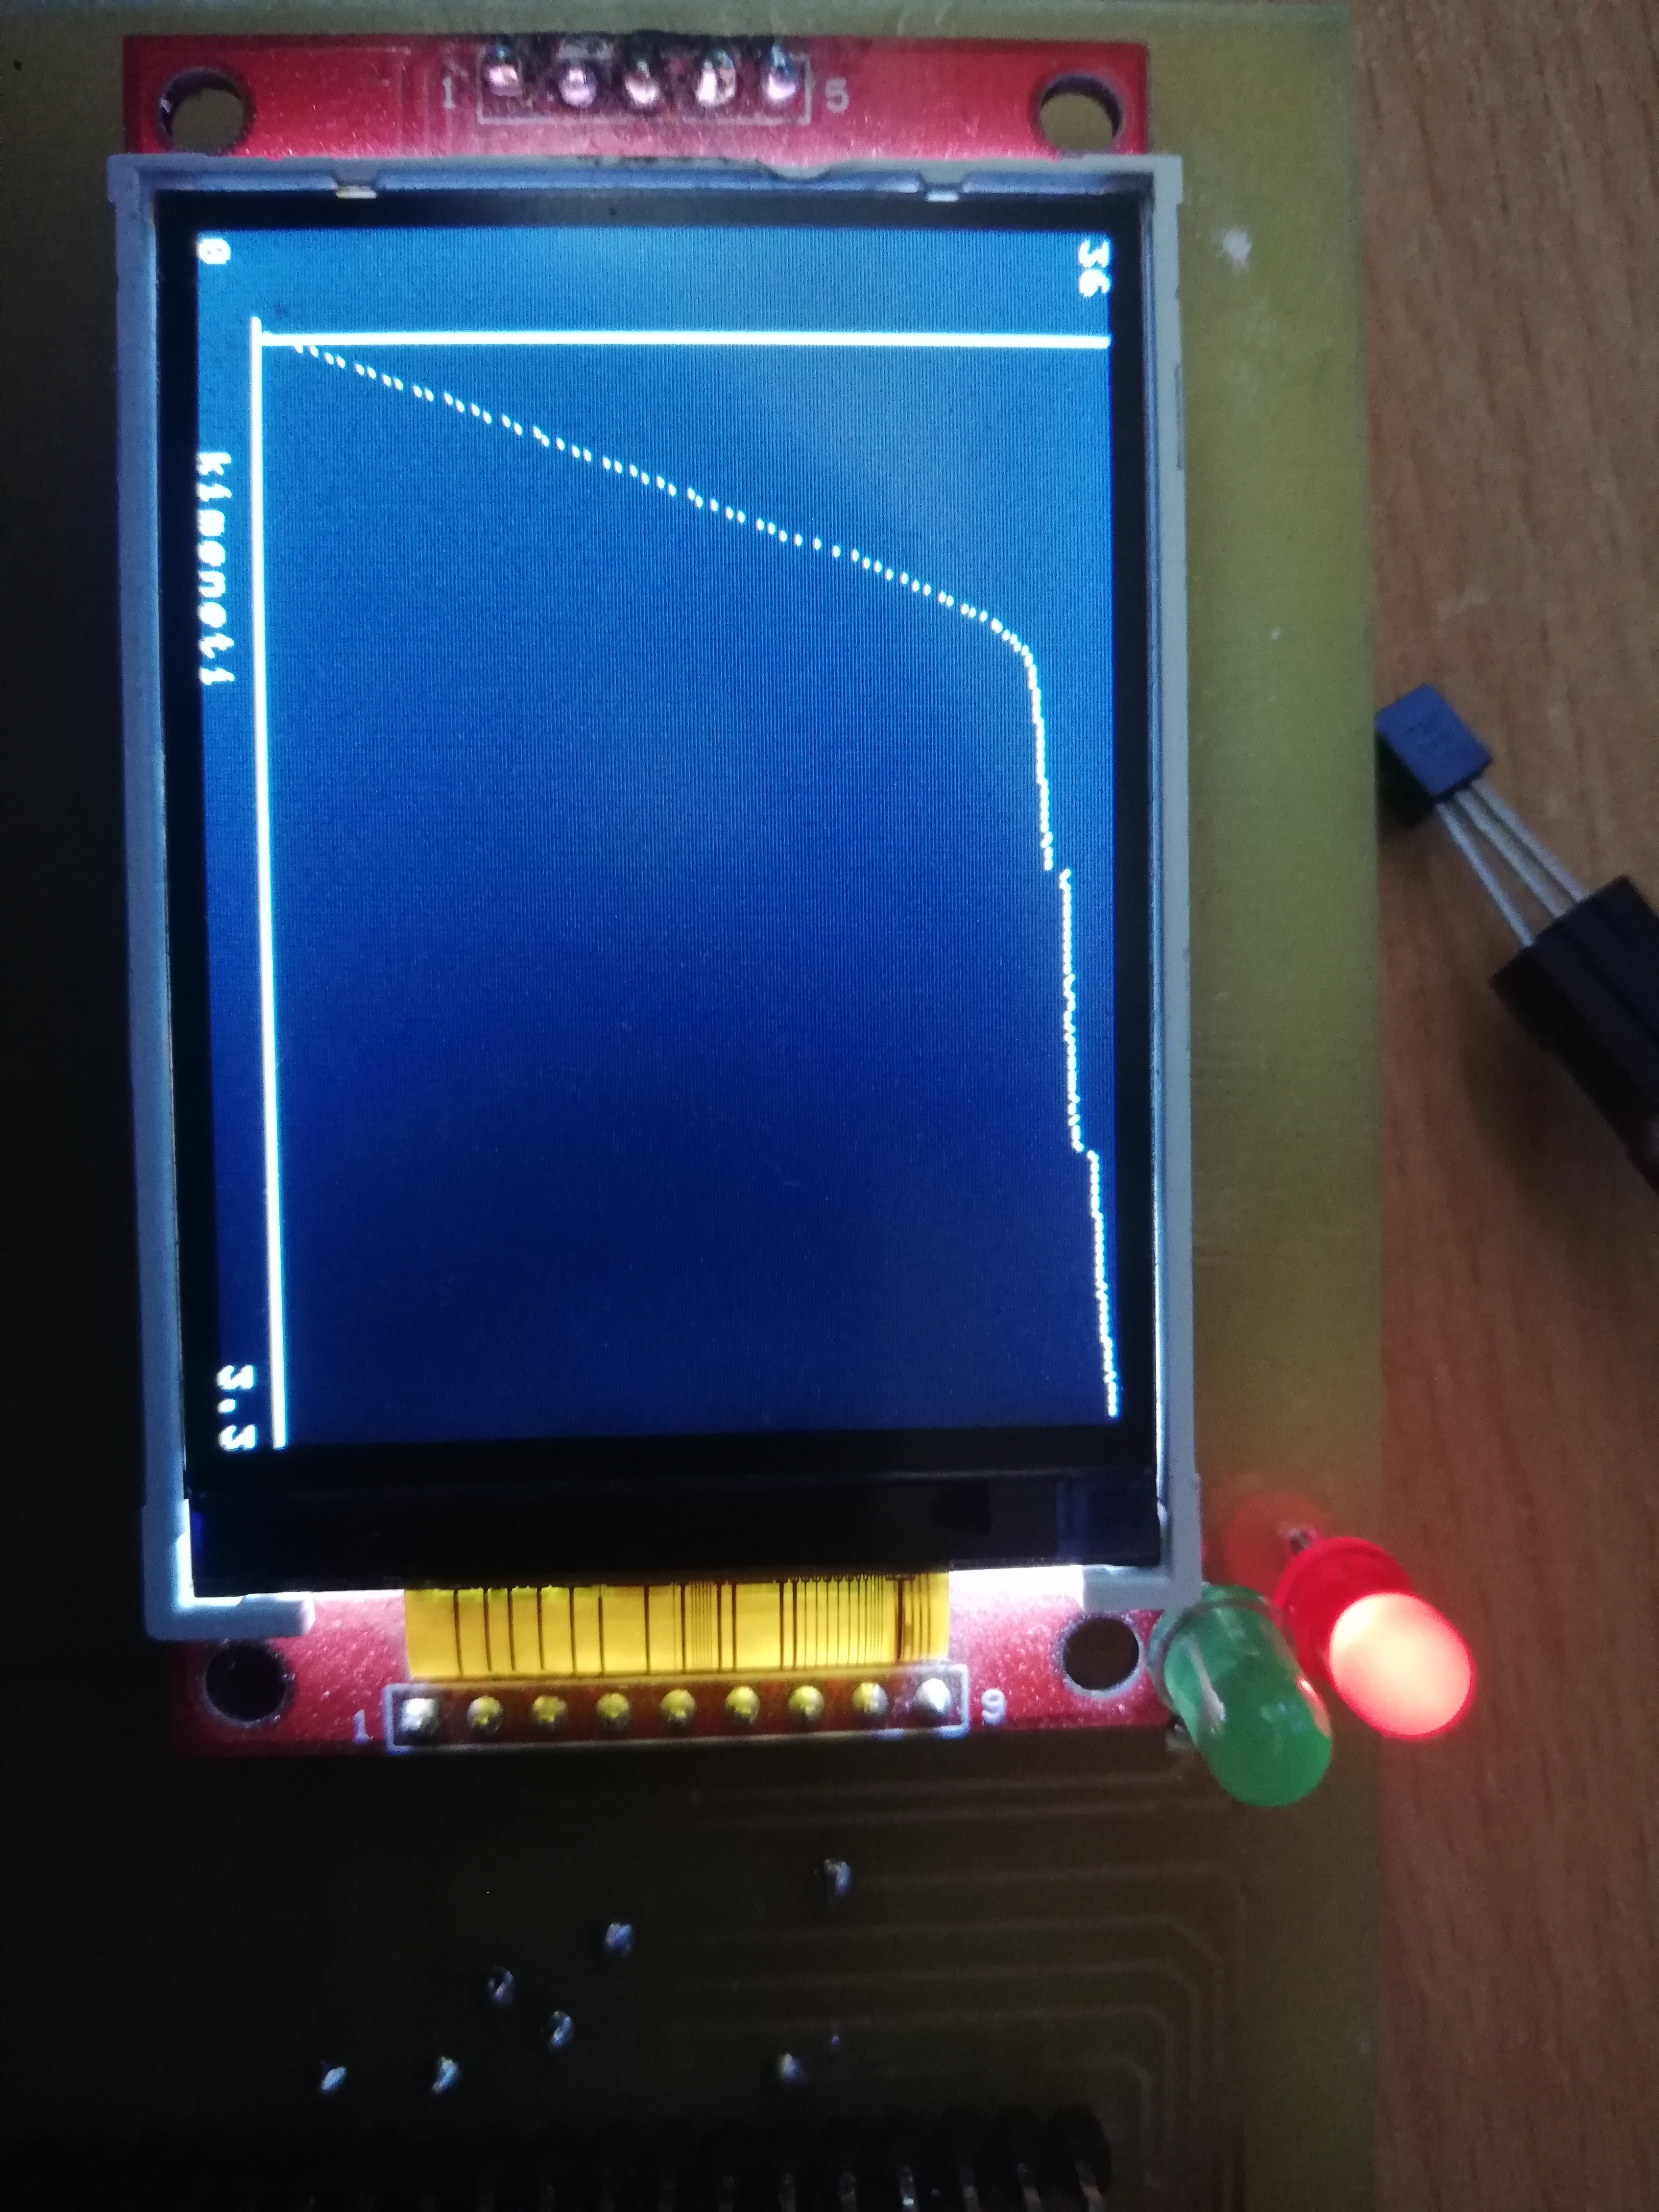
\includegraphics[scale=0.1, angle=90]{images/results/OutChar.jpg}
    \caption{Kimeneti karakterisztika diagram}
    \label{fig:OutChar}
\end{figure}

\subsection{bemeneti karakterisztika}

Ebben az esetben a kollektor és az emitter a földre van kötve,
miközben a bázis feszültség növekedik. A kapcsoló ellenálláson eső feszültségből
kiszámítható az áram. A diagram a dióda karakterisztikához hasonló eredményt
ad.[\ref{fig:InChar}] 

\begin{figure}[H]
    \centering
    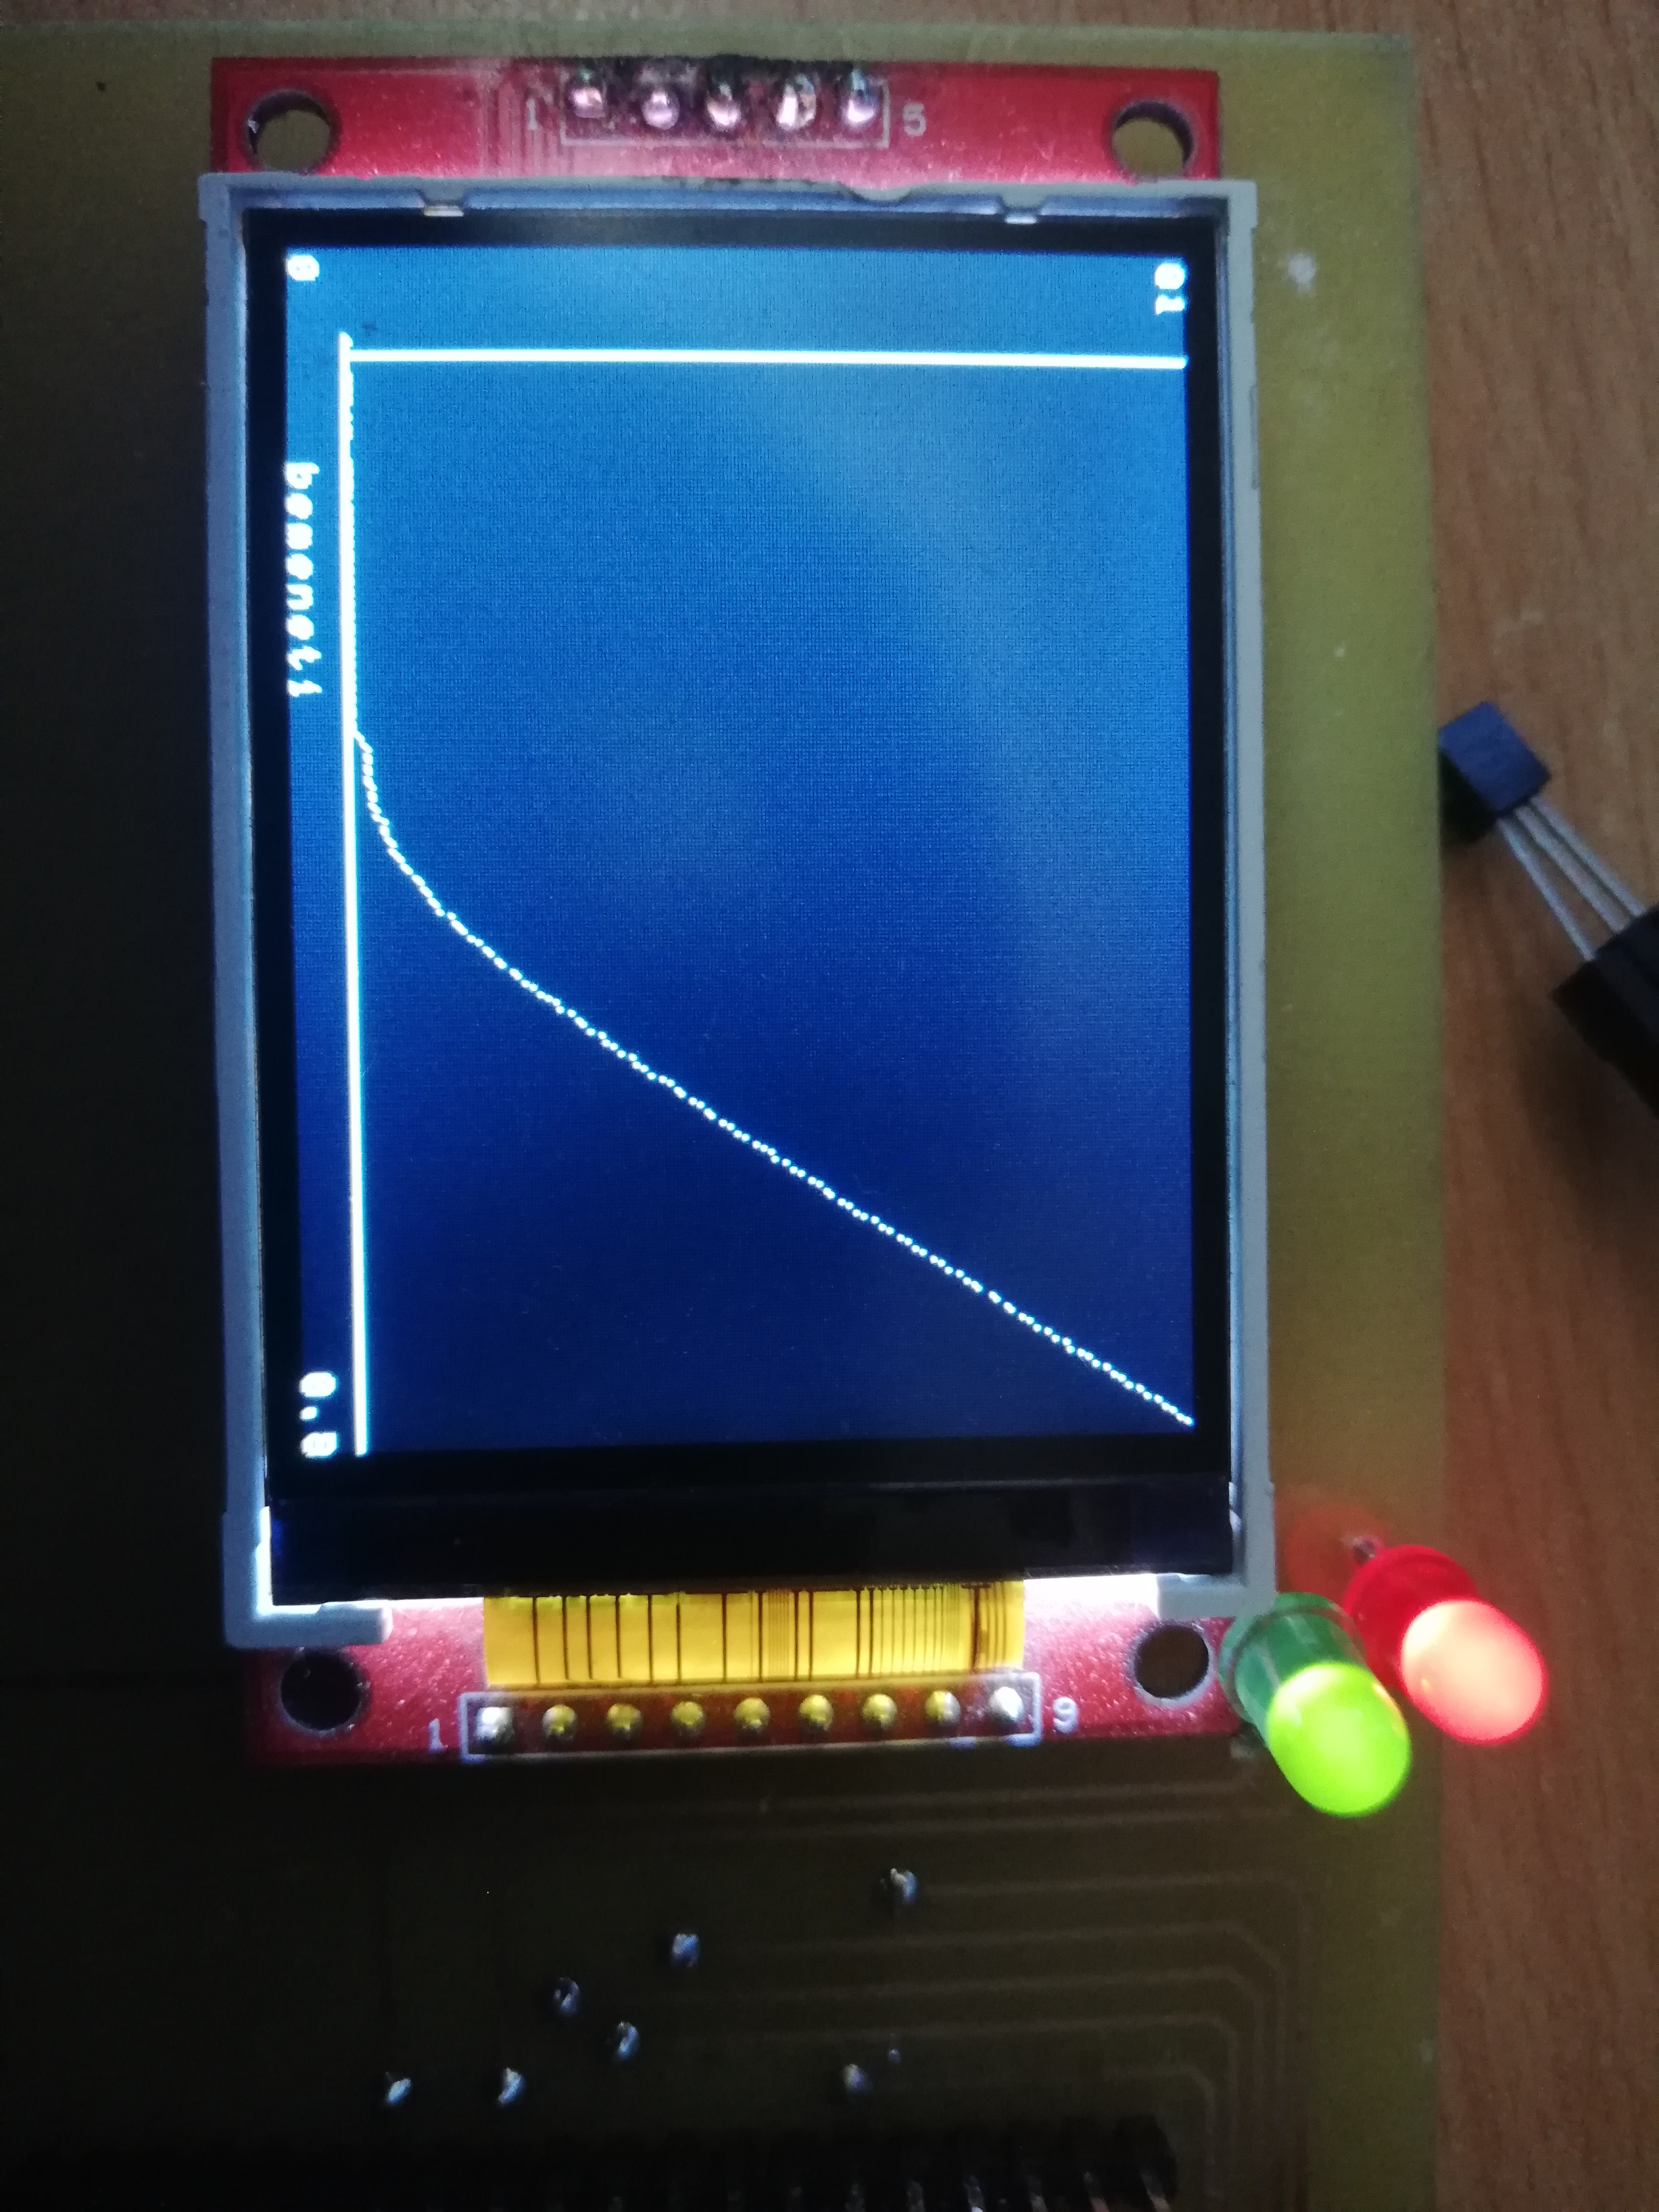
\includegraphics[scale=0.1, angle=90]{images/results/InChar.jpg}
    \caption{Bemeneti karakterisztika diagram}
    \label{fig:InChar}
\end{figure}

